
本章致力于一个特定\trCapacity{}函数的存在性证明，该函数记作 $c_{0}$，%
由 H.~\trHofer{}与 E.~\trZehnder{}在 [123] 中引入。它与\trHamiltonianSystem{}%
的\trPeriodicOrbit{}有着密切的联系。容量 $c_{0}(M,\omega)$ 度量的是特殊的%
\trHamiltonianFunction{} $H:M\to\R$ 的最小 $C^{0}$\textbf{\trOscillation}%
（oscillation）——为了断言存在一个\trPeriodic{}很小、且求解 $M$ 上相应的%
\trHamiltonianSystem{} $X_H$ 的特定\trPeriodicOrbit，就需要这个量。%
对二维\trManifold{}而言，$c_{0}$ 与总面积一致；而在\trConvex{}的、开的且\trSmooth{}的%
\trDomain{} $U\subset(\R^{2n},\omega_{0})$ 这一特殊情形，它由 $\partial U$ 的%
一条特定\trClosedCharacteristic{}所表示，这条\trClosedCharacteristic{}%
具有等于 $c_{0}(U,\omega_{0})$ 的最小（约化）\trAction。例如，由此可以%
展示 $\R^{2n}$ 中的一类\trCompact\trHypersurface，它们与\trConvex{}的\trHypersurface{}并不%
\trSymplectic\trDiffeomorphic。证明将基于\trAction{}原理；这一变分方法将得到%
详细的阐述。我们将在\trSobolev{}空间 $\Hh{1}{2}$ 的分析框架中引入一个特殊的%
\trMinimax{}论证，它起源于 P.~\trRabinowitz{}的工作。$c_{0}$ 的构造补全了%
第 2 章所描述的诸\trSymplectic\trRigidity{}现象的证明；然而，$c_{0}$ 的种种%
特殊性质，对后文\trHamiltonianDynamics{}的研究也将有所助益。

\section{容量\texorpdfstring{$c_{0}$}{c0}的定义}
\label{sec:capacity-c0}

若 $(M,\omega)$ 是一个\trSymplecticManifold，我们回顾：$M$ 上每个\trSmooth{}%
函数 $H:M\to\R$ 都唯一地对应一个\trHamiltonianVectorField{} $X_H$，其定义为
\[
\omega(X_H(x),v)=-dH(x)(v),\qquad v\in T_{x}M,\quad x\in M.
\]
\trHamiltonianEquation
\[
\dot{x}=X_H(x)\qquad\text{在}\ M\ \text{上}
\]
的 $T$-\trPeriodicSolution{} $x(t)$，是指对某个 $T>0$ 满足\trBoundaryCondition{}%
$x(T)=x(0)$ 的解。现在，我们挑出一类特定的\trHamiltonianFunction{} $H$，%
其定性形态如下图 3.1 所绘。

当 $M$ 具有\trBoundary{} $\partial M$ 时，\trHamiltonianVectorField{} $X_H$%
具有\textbf{\trCompactSupport}（compact support），且该\trSupport{}含于 $M$ 的%
\trInterior。我们的指导原则是如下期望：若函数 $H$ 的\trOscillation{}%
充分大，则相应的\trHamiltonianVectorField{}便拥有一个快速的\trPeriodicSolution{}%
——即\trPeriodic{} $T$ 很小（譬如 $0<T\leq1$）的\trPeriodicSolution——%
而与其\trSupport{}的大小无关。

\noindent\begin{minipage}{\linewidth}
\centering
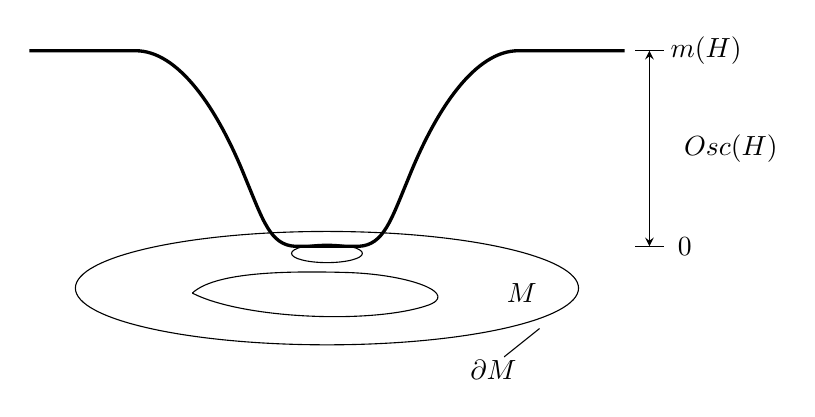
\begin{tikzpicture}[>=stealth,scale=0.9]
  \draw (0,-0.35) ellipse (3.55 and 0.8);%
  \draw (-1.9,-0.42) .. controls (-1.2,-0.78) and (0.6,-0.86) .. (1.4,-0.6)
        .. controls (1.9,-0.44) and (1.2,-0.16) .. (0.3,-0.13)
        .. controls (-0.7,-0.1) and (-1.6,-0.14) .. (-1.9,-0.42);%
  \draw (0,0.14) ellipse (0.5 and 0.13);%
  \draw[very thick] (-4.2,3) -- (-2.7,3)
        .. controls (-2.1,3) and (-1.55,2.2) .. (-1.15,1.2)
        .. controls (-0.9,0.6) and (-0.8,0.26) .. (-0.45,0.24)
        -- (0.45,0.24)
        .. controls (0.8,0.26) and (0.9,0.6) .. (1.15,1.2)
        .. controls (1.55,2.2) and (2.1,3) .. (2.7,3)
        -- (4.2,3);%
  \draw (4.35,3) -- (4.75,3);%
  \draw (4.35,0.24) -- (4.75,0.24);%
  \draw[<->] (4.55,3) -- (4.55,0.24);%
  \node at (5.35,3) {$m(H)$};
  \node at (5.05,0.24) {$0$};
  \node at (5.7,1.62) {$\operatorname{Osc}(H)$};
  \node at (2.75,-0.42) {$M$};
  \node at (2.35,-1.5) {$\partial M$};
  \draw (2.5,-1.32) -- (3.0,-0.92);%
\end{tikzpicture}

图 3.1
\end{minipage}

确切地说，我们用 $\mathcal{H}(M,\omega)$ 表示 $M$ 上满足下列三条性质的%
\trSmooth{}函数 $H$ 全体：

\textbf{P.1.}\ 存在一个\trCompact{}集 $K\subset M$（依赖于 $H$），使得%
$K\subset(M\setminus\partial M)$，并且
\[
H(M\setminus K)\equiv m(H)\quad\text{（常数）}
\]

\textbf{P.2.}\ 存在一个\trOpenSet{} $U\subset M$（依赖于 $H$），使得
\[
H(U)\equiv 0
\]

\textbf{P.3.}\ 对一切 $x\in M$ 有 $0\leq H(x)\leq m(H)$。

常数 $m(H)=\max H-\min H$ 称为 $H$ 的\trOscillation。若 $M$ 上%
$\dot{x}=X_H(x)$ 的一切\trPeriodicSolution{}都是常值的（即对一切 $t$ 有%
$x(t)\equiv x(0)$），或者其\trPeriodic{} $T>1$，则称 $H\in\mathcal{H}(M,\omega)$%
为\trAdmissible{}的（admissible）。把\trAdmissible{}函数全体简记为%
$\mathcal{H}_{a}(M,\omega)\subset\mathcal{H}(M,\omega)$，我们定义
\[
c_{0}(M,\omega)=\sup\ \bigl\{\,m(H)\ \bigm|\ H\in\mathcal{H}_{a}(M,\omega)\,\bigr\}.
\]

于是，若 $c_{0}(M,\omega)<\infty$，则这个数由下述性质所刻画：对%
$\mathcal{H}(M,\omega)$ 中每个\trOscillation{}满足 $m(H)>c_{0}(M,\omega)$ 的%
函数 $H$，\trVectorField{} $X_H$ 便对某个 $0<T\leq1$ 拥有一个非常值的%
$T$-\trPeriodicSolution；而 $c_{0}(M,\omega)$ 正是具有这一性质的诸实数之下确界。%
本章的主要结果是

\begin{theorem}\label{thm:c0-capacity}
函数 $c_{0}$ 是一个\trSymplecticCapacity。此外，$c_{0}=\check{c}_{0}$，%
即 $c_{0}$ 具有\trInnerRegularity。
\end{theorem}

作为说明，我们考察 $(\R^{2n},\omega_{0})$ 中由诸不变量%
$r_{1}(E)\leq r_{2}(E)\leq\dots\leq r_{n}(E)$ 所确定的\trEllipsoid{} $E$。%
我们知道，对每个\trCapacity{} $c$ 都有 $c(E,\omega_{0})=\pi r_{1}(E)^{2}$。%
于是，这个线性不变量可以动态地定义如下：

\begin{proposition}\label{prop:ellipsoid-dynamic}
若 $H\in\mathcal{H}(E,\omega_{0})$ 满足 $m(H)>\pi r_{1}(E)^{2}$，则 $E$ 上的%
\trHamiltonianVectorField{} $X_H$ 拥有非常值的\trPeriodicSolution，其%
\trPeriodic{}满足 $0<T\leq1$。此外，$\pi r_{1}(E)^{2}$ 便是具有此性质的%
诸实数之下确界。
\end{proposition}

\begin{corollary}\label{cor:ball-oscillation}
若 $H\in\mathcal{H}(B(r),\omega_{0})$ 满足
\[
m(H)>\pi r^{2},
\]
则\trHamiltonianSystem{} $\dot{x}=X_H(x)$ 在 $B(r)$ 上拥有非常值的%
\trPeriodicSolution，其\trPeriodic{}满足 $0<T\leq1$。
\end{corollary}

首先注意，关于\trInnerRegularity{}的论断%
$c_{0}(M,\omega)=\check{c}_{0}(M,\omega)$ 可由诸定义立即得出。我们只考虑%
$c_{0}(M,\omega)<\infty$ 的情形，$c_{0}(M,\omega)=\infty$ 的情形可类似处理。%
若 $\varepsilon>0$，则存在 $H\in\mathcal{H}_{a}(M,\omega)$ 使得%
$m(H)>c_{0}(M,\omega)-\varepsilon$。令 $K=\operatorname{supp}(X_H)\subset%
(M\setminus\partial M)$，并取\trOpenSet{} $U$ 使得%
$K\subset U\subset\overline{U}\subset(M\setminus\partial M)$。显然%
$H\in\mathcal{H}_{a}(U,\omega)$，从而 $c_{0}(U,\omega)\geq%
c_{0}(M,\omega)-\varepsilon$，于是
\[
c_{0}(M,\omega)=\sup\bigl\{\,c_{0}(U,\omega)\ \bigm|\ U\subset M\ \text{开，且}\
\overline{U}\subset M\setminus\partial M\,\bigr\},
\]
而由定义，这正等于 $\check{c}_{0}(M,\omega)$。

我们还须证明 $c_{0}(M,\omega)$ 满足一个\trCapacity{} $c$ 的诸公理；%
为方便读者，在此把这些公理回顾一遍。所考察的一切\trSymplecticManifold{}%
都具有固定的维数 $2n$。

\textbf{A1. \trMonotonicity}：只要存在\trSymplecticEmbedding{}%
$\varphi:M\to N$，便有 $c(M,\omega)\leq c(N,\sigma)$。

\textbf{A2. \trConformality}：$c(M,\alpha\omega)=|\alpha|\,c(M,\omega)$，%
其中 $\alpha\neq0$。

\textbf{A3. \trNormalization}：$c(Z(1),\omega_{0})=\pi=c(B(1),\omega_{0})$。

前两条性质由 $c_{0}$ 的定义极易得出。

\begin{lemma}\label{lem:monotonicity-axiom}
$c_{0}$ 满足\trMonotonicity{}公理 (A1)。
\end{lemma}
\begin{proof}
若 $\varphi:M\to N$ 是一个\trSymplecticEmbedding，我们可如下定义映射%
$\varphi_{*}:\mathcal{H}(M,\omega)\to\mathcal{H}(N,\sigma)$：
\[
\varphi_{*}(H)=
\begin{cases}
H\circ\varphi^{-1}(x) & \text{若}\quad x\in\varphi(M),\\[4pt]
m(H) & \text{若}\quad x\notin\varphi(M).
\end{cases}
\]
注意，若 $K\subset M$ 为\trCompact{}集且 $K\subset M\setminus\partial M$，%
则也有 $\varphi(K)\subset N\setminus\partial N$，故确实有%
$\varphi_{*}(H)\in\mathcal{H}(N,\sigma)$。显然 $m(\varphi_{*}(H))=m(H)$，%
于是只要证明 $\varphi_{*}\bigl(\mathcal{H}_{a}(M,\omega)\bigr)\subset%
\mathcal{H}_{a}(N,\sigma)$，引理便得证。由于 $\varphi$ 是\trSymplectic{}的，%
在 $\varphi(M)$ 上有 $\varphi_{*}(X_H)=X_{\varphi_{*}(H)}$，从而诸\trFlow{}%
相互\trConjugate。特别地，非常值\trPeriodicSolution{}连同其\trPeriodic{}%
彼此一一对应。
\end{proof}

\begin{lemma}\label{lem:conformality-axiom}
$c_{0}$ 满足\trConformality{}公理 (A2)。
\end{lemma}
\begin{proof}
设 $\alpha\neq0$，并定义显然的双射%
$\psi:\mathcal{H}(M,\omega)\to\mathcal{H}(M,\alpha\omega)$：%
$\psi:H\mapsto|\alpha|\cdot H=H_{\alpha}$。显然 $m(H_{\alpha})=|\alpha|\cdot m(H)$，%
于是只要证明 $\psi$ 在 $\mathcal{H}_{a}(M,\omega)$ 与%
$\mathcal{H}_{a}(M,\alpha\omega)$ 之间也是双射，引理便得证。由%
\trHamiltonianVectorField{}的定义，
\[
(\alpha\omega)(X_{H_{\alpha}},\cdot)=-dH_{\alpha}=-|\alpha|\,dH=|\alpha|\ %
\omega(X_{H},\cdot).
\]
从而，由于 $\omega$ 是\trNondegenerate{}的，
\[
\frac{\alpha}{|\alpha|}\,X_{H_{\alpha}}=X_{H}\qquad\text{在}\ M\ \text{上}.
\]
因此 $X_{H_{\alpha}}=X_H$ 或 $X_{H_{\alpha}}=-X_H$，两个\trVectorField{}%
具有相同的\trPeriodicSolution{}与相同的\trPeriodic。
\end{proof}

\begin{lemma}\label{lem:ball-ge-pi}
$c_{0}(B(1),\omega_{0})\geq\pi$。
\end{lemma}
\begin{proof}
取 $0<\varepsilon<\pi$。我们将构造一个函数 $H\in\mathcal{H}_{a}(B(1))$%
满足 $m(H)=\pi-\varepsilon$，从而证明 $c_{0}(B(1),\omega_{0})\geq\pi-\varepsilon$。%
选取\trSmooth{}函数 $f:[0,1]\to[0,\infty)$ 使其满足
\begin{align*}
0\leq\ &f'(t)<\pi,\\
&f(t)=0\quad\text{对}\ t\ \text{靠近}\ 0,\\
&f(t)=\pi-\varepsilon\quad\text{对}\ t\ \text{靠近}\ 1.
\end{align*}

\noindent\begin{minipage}{\linewidth}
\centering
\begin{tikzpicture}[>=stealth,x=3.1cm,y=1.05cm]
  \draw[->] (0,0) -- (1.45,0);%
  \draw[->] (0,0) -- (0,3.6);%
  \node at (0.14,3.72) {$f$};
  \draw (0,3) -- (1,3) -- (1,0);%
  \draw[very thick] (0,0.05)
        .. controls (0.3,0.08) and (0.55,0.5) .. (0.75,1.35)
        .. controls (0.9,2.05) and (0.86,2.72) .. (1,2.75);%
  \draw[dashed] (0,2.75) -- (1,2.75);%
  \draw (-0.03,3) -- (0.03,3);%
  \node[left] at (-0.05,3) {$\pi$};
  \node[left] at (-0.05,2.75) {$\pi-\varepsilon$};
  \node[below left] at (0,0) {$0$};
  \draw (1,-0.04) -- (1,0.04);
  \node[below] at (1,-0.07) {$1$};
  \node[below] at (1.38,0) {$t$};
\end{tikzpicture}

图 3.2
\end{minipage}

对 $x\in B(1)$ 定义 $H(x)=f(|x|^{2})$。则 $m(H)=\pi-\varepsilon$，而且我们%
断言 $H\in\mathcal{H}_{a}(M,\omega)$。事实上，\trHamiltonianSystem
\[
-J\dot{x}=\nabla H(x)=2f'(|x|^{2})x
\]
以函数 $G(x)=\frac{1}{2}|x|^{2}$ 为\trFirstIntegral，这是因为%
$\langle\nabla G,J\nabla H\rangle=2f'(|x|^{2})\langle x,Jx\rangle=0$。于是，%
若 $x(t)$ 是一个解，则
\[
2f'\bigl(|x(t)|^{2}\bigr)=a
\]
为常数，并且该解满足
\[
-J\dot{x}=ax.
\]
从而，所有的解都是周期的，且由 $x(t)=e^{aJt}x(0)=(\cos at)x(0)+(\sin at)Jx(0)$%
给出。若 $a=0$，则解为常值的；而若 $a>0$，则\trPeriodic{}为%
$T=\frac{2\pi}{a}>1$，因为由构造有 $0\leq a<2\pi$。因此，正如我们所要证明的，%
$H$ 是\trAdmissible{}的。
\end{proof}

包含映射 $B(1)\to Z(1)$ 是一个\trSymplecticEmbedding，于是由%
\cref{lem:monotonicity-axiom}与\cref{lem:ball-ge-pi}得到
\[
c_{0}(Z(1))\geq c_{0}(B(1))\geq\pi.
\]

为了证明 $c_{0}$ 满足\trNormalization{}公理 (A3)，我们还须证明%
$c_{0}(Z(1))\leq\pi$。这是证明中微妙的部分：它需要一个存在性证明，%
而我们的下一个目标便是证明

\begin{theorem}\label{thm:z1-period-1}
若 $H\in\mathcal{H}(Z(1))$ 满足 $m(H)>\pi$，则 $Z(1)$ 上的%
\trHamiltonianSystem{} $\dot{x}=J\nabla H(x)$ 拥有位于 $Z(1)$ 内、%
\trPeriodic{}为 $T=1$ 的\trPeriodicSolution，并且它不是常值解。
\end{theorem}

这个定理在本质上是定性的。我们观察到，在证明\cref{thm:z1-period-1}时，%
可以把 $H$ 换成 $H\circ\psi$，其中 $\psi$ 是 $Z^{2n}(1)$ 的一个%
\trCompactSupport{}\trSymplecticDiffeomorphism，即集合%
$\{x\mid\psi(x)\neq x\}$ 的\trClosure{}是 $Z^{2n}(1)$ 的一个\trCompact{}子集。%
的确，鉴于\trHamiltonianVectorField{}的\trTransformationLaw{}（transformation law，第 1 章），$X_H$ 与%
$X_{H\circ\psi}$ 的诸\trFlow{}相互\trConjugate。利用这一观察，我们可以不失%
一般性地假设 $H$ 在原点的一个\trNeighborhood{}内为零。这证明如下。%
由假设 $H|_{U}\equiv0$。我们取一点 $z_{0}\in U$，并选取\trSmooth{}函数%
$\rho:\R^{2n}\to\R$，它在 $Z^{2n}(1)$ 内具有\trCompactSupport，并且在连接%
原点与 $z_{0}$ 的直线 $\{tz_{0}\mid 0\leq t\leq1\}$ 的一个\trNeighborhood{}%
$V$ 上等于 $1$。定义\trHamiltonianFunction{} $K:Z^{2n}(1)\to\R$ 为
\[
K(z)=\rho(z)\langle z,-Jz_{0}\rangle\ .
\]
于是，$X_K$ 的\trTimeOneMap{} $\psi$ 是\trSymplectic{}的，且在 $Z^{2n}(1)$ 内%
具有\trCompactSupport。由于当 $z\in V$ 时 $X_K(z)=z_{0}$，直线%
$\psi^{t}(0)=tz_{0}$ 便是对 $0\leq t\leq1$ 而言的一个解，它把原点移动到点%
$z_{0}$。因此
\[
\psi(0)=z_{0}\ ,
\]
而\trHamiltonianFunction{} $H\circ\psi$ 在 $0$ 的一个\trNeighborhood{}内为零。

因此，从现在起我们假设\trHamiltonianFunction{} $H$ 在原点的一个开%
\trNeighborhood{}内为零，并先把定义在 $Z(1)$ 上的 $H$ \trContinuation{}成整个空间%
$\R^{2n}$ 上定义的函数。这当然是容易的，因为该函数在 $Z(1)$ 的\trBoundary{}%
附近是常数。然而，考虑到后面的证明，我们将选取一个非常特殊的\trContinuation。%
首先注意，若 $H\in\mathcal{H}(Z(1),\omega_{0})$，则存在一个\trEllipsoid{}%
$E=E_{N}$ 使得 $H\in\mathcal{H}(E,\omega_{0})$，其中
\[
E_{N}=\bigl\{\,z\in\R^{2n}\ \bigm|\ q(z)<1\,\bigr\},
\]
其在坐标 $z=(x,y)$ 之下由
\[
q(z)=\bigl(x_{1}^{2}+y_{1}^{2}\bigr)+\frac{1}{N^{2}}\sum_{j=2}^{n}%
\bigl(x_{j}^{2}+y_{j}^{2}\bigr)
\]
给出，而 $N\in\Z^{+}$ 取得充分大（图 3.3）。

\noindent\begin{minipage}{\linewidth}
\centering
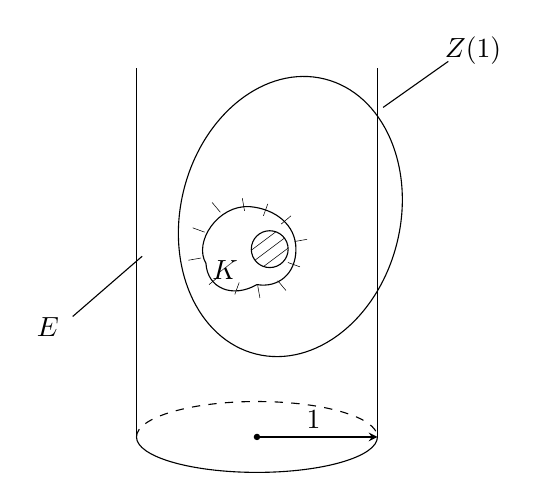
\begin{tikzpicture}[>=stealth,scale=0.9]
  \draw (-1.7,4.6) -- (-1.7,-0.6);%
  \draw (1.7,4.6) -- (1.7,-0.6);%
  \draw[dashed] (-1.7,-0.6) arc (180:0:1.7 and 0.5);%
  \draw (-1.7,-0.6) arc (180:360:1.7 and 0.5);%
  \fill (0,-0.6) circle (1.3pt);
  \draw[->] (0,-0.6) -- (1.7,-0.6);%
  \node at (0.8,-0.36) {$1$};
  \begin{scope}[rotate=-14]
    \draw (-0.15,2.55) ellipse (1.55 and 2.0);%
  \end{scope}
  \draw (-0.1,2.65) .. controls (0.25,2.62) and (0.55,2.4) .. (0.55,2.05)
        .. controls (0.55,1.7) and (0.3,1.5) .. (0.0,1.55)
        .. controls (-0.35,1.35) and (-0.7,1.5) .. (-0.72,1.85)
        .. controls (-0.9,2.15) and (-0.55,2.68) .. (-0.1,2.65);%
  \foreach \a/\r in {10/0.62,40/0.55,70/0.5,100/0.55,130/0.68,160/0.7,190/0.72,220/0.6,250/0.5,280/0.52,310/0.58,340/0.55}
    \draw[very thin] ([shift={(-0.08,2.05)}]\a:\r) -- ++(\a:0.18);%
  \begin{scope}%
    \clip (0.18,2.05) circle (0.26);
    \foreach \d in {-0.36,-0.18,0,0.18,0.36}
      \draw[very thin] (-0.3,1.69+\d) -- (0.66,2.41+\d);
  \end{scope}
  \draw (0.18,2.05) circle (0.26);
  \node at (3.05,4.85) {$Z(1)$};
  \draw (2.7,4.7) -- (1.78,4.05);%
  \node at (-2.95,0.95) {$E$};
  \draw (-2.6,1.1) -- (-1.62,1.95);%
  \node at (-0.45,1.75) {$K$};
\end{tikzpicture}

图 3.3
\end{minipage}

由于 $H\in\mathcal{H}(Z(1),\omega_{0})$ 满足 $m(H)>\pi$，故存在%
$\varepsilon>0$ 使得 $m(H)>\pi+\varepsilon$。于是，我们可以选取\trSmooth{}%
函数 $f:\R\to\R$ 使其满足
\begin{align*}
f(s)\ &=\ m(H) && \text{对}\ s\leq1\\
f(s)\ &\geq\ (\pi+\varepsilon)s && \text{对一切}\ s\in\R\\
f(s)\ &=\ (\pi+\varepsilon)s && \text{对充分大的}\ s\\
0<f'(s)\ &\leq\ \pi+\varepsilon && \text{对}\ s>1\quad\text{（图 3.4）}.
\end{align*}

\noindent\begin{minipage}{\linewidth}
\centering
\begin{tikzpicture}[>=stealth,x=2.9cm,y=0.95cm]
  \draw[->] (0,0) -- (1.66,0);%
  \draw[->] (0,0) -- (0,4.9);%
  \node at (0.14,5.05) {$f$};
  \node[below] at (1.58,0) {$s$};
  \draw (0,0) -- (2.55,4.2);%
  \draw[very thick] (0,2.6) -- (0.92,2.6)
        .. controls (1.6,2.6) and (2.1,3.46) .. (2.55,4.2) -- (2.75,4.53);%
  \draw[dashed] (0,1.65) -- (1,1.65);%
  \draw[dashed] (1,0) -- (1,1.65);%
  \node[left] at (-0.05,2.6) {$m(H)$};
  \node[left] at (-0.05,1.65) {$\pi+\varepsilon$};
  \node[below left] at (0,0) {$0$};
  \draw (1,-0.06) -- (1,0.06);
  \node[below] at (1,-0.1) {$1$};
\end{tikzpicture}

图 3.4
\end{minipage}

于是，$H$ 的\trContinuation{}由下式定义：
\[
\overline{H}(z)=
\begin{cases}
H(z) & z\in E,\\[4pt]
f(q(z)) & z\notin E.
\end{cases}
\]
显然 $\overline{H}\in C^{\infty}(\R^{2n})$，并且 $\overline{H}$ 在无穷远处是%
二次的：
\[
\overline{H}(z)=(\pi+\varepsilon)q(z),\qquad\text{若}\ |z|\geq R,
\]
其中 $R$ 充分大。下面的关键命题描述了我们所要寻找的那些特定的%
\trPeriodicSolution。

\begin{proposition}\label{prop:phi-positive-in-E}
设 $x(t)$ 是 $\dot{x}=X_{\overline{H}}(x)$ 的\trPeriodic{}为 $1$ 的一个%
\trPeriodicSolution。若它满足
\[
\Phi(x):=\int_{0}^{1}\Bigl\{\frac{1}{2}\langle-J\dot{x},x\rangle-%
\overline{H}(x(t))\Bigr\}\,dt>0,
\]
则 $x(t)$ 为非常值，且 $x(t)\subset E$。从而 $x(t)$ 是原系统%
$\dot{x}=X_H(x)$ 在 $Z(1)$ 上的一个非常值的 $1$-\trPeriodicSolution。
\end{proposition}

\begin{proof}
若 $x(t)=x^{*}$ 是常值解，则因 $\overline{H}\geq0$ 有 $\Phi(x^{*})\leq0$。%
\trHamiltonianVectorField{} $X_{\overline{H}}$ 在 $\partial E$ 上为零。因此，%
若对某个 $t_{0}$ 有 $x(t_{0})\notin E$，则对一切 $t\in\R$ 都有 $x(t)\notin E$，%
从而它求解方程
\[
-J\dot{x}=\nabla\overline{H}(x)=f'(q(x))\cdot\nabla q(x).
\]
注意，在 $E$ 之外，函数 $q$ 是此方程的一个\trFirstIntegral，这是因为%
$\langle\nabla q,Jf'(q)\nabla q\rangle=f'(q)\langle\nabla q,J\nabla q\rangle=0$。%
从而，若 $x(t)$ 是一个解，则
\[
q(x(t))=q(x(t_{0}))=\tau
\]
关于 $t$ 为常数；于是，鉴于 $\langle\nabla q(z),z\rangle=2q(z)$（%
$z\in\R^{2n}$），我们可以算出
\begin{align*}
\Phi(x)\ &=\ \int_{0}^{1}\Bigl\{\frac{1}{2}\langle-J\dot{x},x\rangle-%
\overline{H}(x)\Bigr\}\,dt\\
&=\ \int_{0}^{1}\frac{1}{2}f'(\tau)\langle\nabla q(x),x\rangle\,dt-%
\int_{0}^{1}f(q(x))\,dt\\
&=\ \frac{1}{2}\int_{0}^{1}f'(\tau)\,2q(x(t))\,dt-f(\tau)\\
&=\ f'(\tau)\cdot\tau-f(\tau).
\end{align*}
由 $f$ 的定义，这小于或等于 $(\pi+\varepsilon)\tau-(\pi+\varepsilon)\tau=0$。%
于是，对 $E$ 之外的一切解都有 $\Phi(x)\leq0$，命题得证。
\end{proof}

鉴于这一注记，我们还须找出\trHamiltonianSystem{} $\dot{x}=X_{\overline{H}}(x)$%
的、满足 $\Phi(x)>0$ 的一个 $1$-\trPeriodicSolution{} $x=x(t)$。以下我们将%
改变记号，把 $\overline{H}$ 换写为 $H$。为了建立\trPeriodicSolution{}的%
存在性，我们将利用一个人所共知的\trVariationalPrinciple，其\trCriticalPoint{}%
恰是所需的\trPeriodicSolution。为了引入这一原理，我们暂且在非正式的层面上%
进行，考察\textbf{\trLoopSpace}（loop space）
\[
\Omega=C^{\infty}(S^{1},\R^{2n}),\qquad\text{其中}\ S^{1}=\R/\Z,
\]
即 $\R^{2n}$ 中\trSmooth{}\trLoop{}全体。我们如下定义一个函数%
$\Phi:\Omega\to\R$：
\[
\Phi(x)=\int_{0}^{1}\frac{1}{2}\langle-J\dot{x},x\rangle\,dt-%
\int_{0}^{1}H(x(t))\,dt,\qquad x\in\Omega,
\]
并断言：$\Phi$ 的诸\trCriticalPoint{}便是 $\dot{x}=X_H(x)$ 的诸%
\trPeriodicSolution。在点 $x\in\Omega$ 处沿方向 $y\in\Omega$ 计算其导数，%
我们得到
\begin{align*}
\Phi'(x)(y)\ &=\ \frac{d}{d\varepsilon}\,\Phi(x+\varepsilon y)%
\Big|_{\varepsilon=0}\\
&=\ \int_{0}^{1}\langle-J\dot{x}-\nabla H(x),y\rangle\,dt.
\end{align*}
从而，$\Phi'(x)(y)=0$ 对一切 $y\in\Omega$ 成立当且仅当\trLoop{} $x$ 满足方程
\[
-J\dot{x}(t)-\nabla H(x(t))=0,
\]
即 $x(t)$ 是\trHamiltonianEquation{}的一个解，并且还满足 $x(0)=x(1)$，%
故它是\trPeriodic{}为 $1$ 的\trPeriodicSolution。于是，这一原理在%
\trHamiltonianVectorField{}的全部解所构成的纷繁集合中，恰好挑选出%
$1$-\trPeriodicSolution。这一原理就是力学中众所周知的\trAction{}原理，%
在力学中人们常用它来推导\trHamiltonianVectorField{}的\trTransformationLaw。%
利用这一原理来做存在性证明，乍看之下或许显得相当别扭，因为它是高度%
\trDegenerate{}的。的确，取特殊的\trLoop{} $x_{j}$：
\[
x_{j}(t)=e^{j2\pi Jt}\xi=(\cos j2\pi t)\xi+(\sin j2\pi t)J\xi,
\]
其中 $|\xi|=1$，对 $\Phi$ 的第一部分我们容易算出
\[
\int_{0}^{1}\frac{1}{2}\langle-J\dot{x}_{j},x_{j}\rangle\,dt=\pi j,\qquad%
\|x_{j}\|_{L_{2}}=1,
\]
而 $\Phi$ 的第二部分却保持有界。我们看到，这个\trFunctional{}既非%
\trBoundedBelow{}亦非\trBoundedAbove。特别地，基于\trMinimizingSequence{}的%
诸变分技巧在此并不适用。这与\trRiemann{}\trManifold{}上\trClosed\trGeodesic{}的%
\trVariationalPrinciple{}恰成鲜明的对照。这一几何问题催生了两种强有力的%
变分方法，即所谓的\trMorseTheory{}与\trLjusternik-\trSchnirelman{}理论。%
我们还应指出，\trMorseTheory{}并不能直接应用于我们的\trFunctional。%
的确，诸\trCriticalPoint{}的\trMorseIndex{}先验地为无穷，从而在拓扑上%
不可见。正是这一困难迫使 Andreas~\trFloer{}去发展扩充\trMorseTheory{}的强有力%
新技术，这使他走向了后文将更详细描述的所谓的 \trFloer{}复形。

直到相对晚近，P.~\trRabinowitz{}[180, 181] 才证明了这一\trDegenerate{}的%
\trVariationalPrinciple{}能够非常有效地用于存在性证明。为此目的，他引入了%
适配于\trFunctional{} $\Phi$ 之结构的特殊\trMinimax{}原理。在我们描述这些%
技术细节之前，先在一个抽象的框架中回顾一下\trMinimax{}思想，或许不无助益。
